\documentclass{emulateapj}
%\documentclass[12pt,preprint]{aastex}

\usepackage[utf8]{inputenc}
\usepackage{graphicx}
\usepackage{float}
\usepackage{amsmath}
\usepackage{epsfig,floatflt}
\usepackage{url}
\setcitestyle{square}

\begin{document}

\title{Modeling the Solar System using object-oriented code to solve differential equations}

\author{Hans Erlend Bakken Glad, Torbjørn Lode Gjerberg, Christer Dreierstad, Stig-Nicolai Foyn}

\email{heglad@student.matnat.uio.o,  torbjolg@student.matnat.uio.no ,stignicf@student.matnat.uio.no, chrisdre@student.matnat.uio.no}

\altaffiltext{1}{Institute of Physics, University of
  Oslo, P.O.\ Box 1029 Blindern, N-0315 Oslo, Norway}

%\date{Received - / Accepted -}

\begin{abstract}
Solving differential equations describing the motion of a planet orbiting a star as a two-body problem is easily solved using simple numerical methods, such as the Euler method. When considering the energy of the system we observe that the Euler method does not conserve energy, as time goes the system gains energy. Further we observe that the angular momentum increases with time using the Euler method. Implementing the Velocity Verlet method we get an energy conserving method that produces better results on fewer steps, at the cost of FLOPS. We observe that Velocity Verlet is slower than the Euler method due to the amount of FLOPS needed by Velocity Verlet, but only by a factor close to two. Expanding on the model adding more planets in orbit is most easily done by object-orientation, making the program do what would have had to be hard coded otherwise. 

When changing the $1/r^2$ dependency of the force in the two-body Earth-Sun system to $1/r^{\beta}$ where $\beta \in [2,3]$ we observe that the Earth is in a bound state for $\beta < 3$. When $\beta = 3$ the Earth leaves the orbit around the Sun. Introducing the three-body problem as a system of the Earth, Jupiter and the Sun, where the latter's position is fixed at the origin we study the stability of the Velocity Verlet method. The stability is studied by changing the mass of Jupiter such that we dramatically change the effect it has on the Earth. With the mass 10 times larger the method is still stable, increasing the mass by a factor of 1000 we observe that the Earth is flung out of orbit around the Sun, with a dependency upon the resolution of the calculations. By increasing the amount of steps Earth stays in orbit. For a solar system consisting of Mercury and the Sun we observe that the perihelion precession is 26'' over a century (100 years).

\end{abstract}
\keywords{planetary movement --- computational science --- methods: Velocity Verlet, Forward Euler}

\section{Introduction}
\label{sec:introduction}
Simulating the orbits of the planets in the Solar System is a suitable problem for making use of object-oriented code. While the two-body problem is straightforward to solve numerically, introducing multiple planets can quickly become tedious if the program is not written for this purpose. This is where object-orientation excels, as it is built upon writing code once and then running it several times for different cases. In practice, this is done by writing classes in C++ and using them to solve various problems.

By solving differential equations for the motion of the Earth around a static Sun, we conclude that implementing more bodies will require the same operation for each body. Setting up an object-oriented code and treating the bodies of the Solar System as objects will allow the the program to handle the repetitive calculations using a single constructor or function. The calculation of the orbits is performed with numerical integration, using the Euler method and the Velocity Verlet method. We will compare the stability of the two methods and how well they conserve physical quantities. 

Having a fully object-oriented code, we will be able to extend our model to include all planets in the Solar System.
%(Demonstrate usefulness of object-oriented code)

\section{Theory and method}
\label{sec:method}

\subsection{Integration methods}
The Euler method (or Forward Euler) is a first-order approximation to the solution of a differential equation. In our case, we want to solve for the position of a planet given its acceleration. This means that we require an analytical expression $f$ for the acceleration $a$, an initial velocity $v$ and position $x$. In the one-dimensional case and with a step length of $h$, the values at the time $t + h$ are then
%
\begin{gather*}
    v_{t + h} = v_{t} + a_{t} \cdot h \\
    x_{t + h} = x_{t} + v_{t} \cdot h \\
    a_{t + h} = f(x_{t+1}) 
\end{gather*}
%
or on discretized form with $n$ points, so that a point in time is represented by $ i = \left[0, 1, \dots n-1 \right]$:
%
\begin{gather*}
    v_{i + 1} = v_i + a_i h \\
    x_{i + 1} = x_i + v_i h \\
    a_{i + 1} = f(x_{i+1}).
\end{gather*}
%
In our program, this procedure is repeated until $t$ reaches the desired simulation time. This method can easily be extended to 2 or 3 spatial dimensions.

The problem with the Euler method is that it does not conserve the mechanical energy of the system, i. e. the sum of the kinetic and potential energy,
%
\begin{equation}
E_{tot} = E_k + U,
\end{equation}
%
is not constant over time. Because we are looking at a system with gravity as the only force, the total energy should be conserved because gravity is a conservative force. This issue may not be noticeable for the first few orbits, but this will eventually (depending on the precision used) cause orbits to deviate significantly from their original shape.

A more suitable way of calculating planetary orbits is through using the Velocity Verlet method. This integration method is symmetric in time, which means that it should conserve the total energy of the system when $h \rightarrow 0$. We implement the Velocity Verlet method with
%
\begin{align*}
    x_{i + 1} & = x_i + v_i h + a_i h^2 \\
    a_{i + 1} & = f(x_{i+1}) \\
    v_{i + 1} & = v_i + \frac{h}{2}\left(a_{i+1} + a_i\right),
\end{align*}
%
and these values are calculated $n$ times with a given precision $h$.

\subsection{Scaling the equations governing the Solar System}
We will consider a model of our Solar System where gravity is the only force present. By Newton's law of gravitation, two celestial bodies with mass $M_1$ and $M_2$ separated by a distance $r$ will both experience a force with magnitude
%
\begin{equation}\label{eq:gforce}
    F_G = \frac{G M_1 M_2}{r^2},
\end{equation}
where $G = 6.67408 \times 10^{-11} \ \textrm{N} \ \textrm{kg}^{-2} \textrm{m}^2$. The direction of this force is then determined by the direction of the position vector:
%
\begin{equation*}
    \Vec{e_r} = \Vec{r}/ r ,
\end{equation*}
%
so that the force vector becomes
%
\begin{equation}
    \Vec{F_G} = \frac{G M_1 M_2}{r^2}\Vec{e_r} = \frac{G M_1 M_2}{r^3}\Vec{r}.
\end{equation}
%
The acceleration experienced by the body with mass $M_1$ is then
%
\begin{equation}\label{eq:accel}
    \Vec{a} = \frac{\vec{F_G}}{M_1} = \frac{G M_2}{r^3}\Vec{r},
\end{equation}
%
and similarly for body 2.

If we consider a 'flat' Solar System with only two dimensions (naming the axes $x$ and $y$), the acceleration can be decomposed into
%
\begin{equation*}
    a_x = \frac{G M_2}{r^2}\cdot\frac{\Delta x}{r}, \quad a_y = \frac{G M_2}{r^2}\cdot\frac{\Delta y}{r},
\end{equation*}
%
where $\Delta_x$ and $\Delta_y$ are the differences in position coordinates $x$ and $y$ between the two bodies. This can easily be extended to include the third dimension (the 'height' of the Solar System) as well. 

In order to make our values easier to work with, we will scale the equations accordingly. We define the Sun to have a mass $M_S = M_\odot = 2\times 10^{30}$ kg and express the other masses (such as planets, moons) as a fraction of $M_\odot$. Distance is measured in terms of astronomical units AU, where $1 \ \textrm{AU} = 1.496 \times 10^{11} \ \textrm{meters}$ and time is measured in years. This is appropriate for the scales we are looking at, since the Earth takes one year to orbit the Sun once at an average distance of 1 AU. The gravitational constant can now be expressed as 
%
\begin{equation*}
G = 4\pi^2 \ \frac{\textrm{AU}^3}{\textrm{yr}^{2}M} 
\end{equation*}
%
where $M$ is the total mass in the system. From this we get the expression that will be used to calculate the acceleration $a$ induced by a body with mass $M$:
%
\begin{equation*}
a = \frac{4\pi^2 M}{r^2}, \ \textrm{with} \ [a] = \frac{\textrm{AU}}{\textrm{yr}^2}.
\end{equation*}


\subsection{Our simplest model: Earth orbiting a stationary Sun}
\label{subsec:simple}

To get an idea on how to produce a realistic model of the Solar System, we will first look at a simple model with only the Earth and the Sun present. Earth's orbit is set to be perfectly circular, while in reality it is slightly elliptical. The velocity of a circular orbit expressed in terms of the radius (or orbital distance) $r$ and period $T$ is
%
\begin{equation*}
    v = \frac{2\pi r}{T}.
\end{equation*}
%
For Earth, we have $r = 1 \ \textrm{AU}$ and $T = 1 \ \textrm{yr}$. Earth's orbital velocity is thus always $2\pi$ AU/yr.

If we do not want to introduce the period of an object in our calculations, we can instead calculate the velocity through Eq.\eqref{eq:accel}. In a perfectly circular orbit, the centripetal acceleration experienced by the orbiting body is $a = v^2/r$. This gives us
%
\begin{gather*}
    \frac{v^2}{r} = \frac{GM_2}{r^2} \\
    \Rightarrow \ v = \sqrt{\frac{G M_2}{r}},
\end{gather*}
%
and in the case of $M_2 = M_\odot$ this gives
%
\begin{equation}\label{eq:circularorbit}
    v = \sqrt{\frac{4\pi^2}{r}}.
\end{equation}
%
In our algorithm we position the Sun in the origin of our coordinate system. This further simplifies our calculations, as the distance between the Sun and Earth is simply defined by the coordinates $(x, y)$ of Earth. To test this simple case, we initialize the position of Earth at $x = 1 \ \textrm{AU}$ and $y = 0$. This means that the initial velocity in the $x$-direction has to be zero, otherwise we would not get a circular orbit. For a counter-clockwise orbit around the Sun, we then need to set the initial velocities to
%
\begin{equation*}
    v_x = 0, \quad v_y = 2\pi.
\end{equation*}
%
The stability of our Euler and velocity Verlet algorithms are then tested using different time steps $h$. By looking at the kinetic and potential energy of the system, we can also determine how well the two algorithms conserve energy. Total energy and angular momentum should be conserved in this system since gravity is the only force present, and gravity is a conservative force. In theory, the Verlet algorithm should perform better than the Euler algorithm in this regard. This is because the Velocity Verlet algorithm is a second-order method, so the global error is already lower than the Euler method. In addition, the total energy in a system solved by the Verlet algorithm will oscillate around the true value of the energy \cite{bib:verlet}, while the Euler method can potentially add energy to the system indefinitely.

For the next models, we will not be using the Euler method due to its lack of precision.

\subsection{Escape velocity of the Earth}

If the Earth were to have a high enough velocity, the planet would escape the gravitational influence of the Sun. The minimum velocity that achieves this is called the escape velocity, and we find the magnitude of this velocity by setting up the total energy before and after escaping. We find the potential energy of Earth through the expression for the gravitational force between Earth and the Sun:
%
\begin{equation*}
    F_G = \frac{G M_\odot M_E}{r^2}.
\end{equation*}
%
For conservative forces, the potential is defined as the integral of the force along a path. This gives us 
%
\begin{align*}
    U & = \int F_G \ dr \\
    & = \int \frac{G M_\odot M_E}{r^2} dr \\
    & = -\frac{G M_\odot M_E}{r}.
\end{align*}
%
The minimum velocity that the Earth needs to escape is found by setting the final velocity (after escaping) to zero. We can also set the potential energy to zero after the planet has escaped, since $r \rightarrow \infty$. The total energy before and after escaping is then 
%
\begin{equation*}
    \frac{1}{2}M_E v^2 -\frac{G M_\odot M_E}{r} = \frac{1}{2}M_E \cdot 0 - 0,
\end{equation*}
%
so that 
%
\begin{equation}
    v^2 =\frac{2G M_\odot}{r} \\
\end{equation}
%
\begin{equation}\label{eq:esc_vel}
     \Rightarrow \ v_{escape} = \sqrt{\frac{2G M_\odot}{r} } = \sqrt{\frac{4\pi^2}{r}}.
\end{equation}
%
This analytical expression can be used to verify if our model is realistic, as we should see a planet escaping if we set its initial velocity to a value higher than $v_{escape}$.


\subsection{Modified Newtonian gravity}
\label{subsec:modified_gravity}

Centripetal forces on the form $F \propto 1/r^2$ (such as Newtonian gravity) have the property that they allow for closed orbits \cite{bib:project3}. After one orbital period, an object with a closed orbit will end up at the same position it started. We modify the $r$-dependency in the model for Newtonian gravity (Eq. \eqref{eq:gforce}) so that
%
\begin{equation}
    F_G = \frac{G M_1 M_2}{r^\beta}, \quad \beta \in \left[2,3\right].
\end{equation}
%
We will study the effects of using this modified gravitational force, specifically in the model outlined in section \ref{subsec:simple}. Running a simulation of Earth orbiting the Sun with $\beta > 2$ should cause the Earth to no longer have a closed orbit. This effect should become more clear when $\beta \rightarrow 3$, as the gravitational force will weaken accordingly.


\subsection{Expanding our model: Adding Jupiter to the system}

After object-orienting our code, adding more planets should only be a matter of introducing new objects that represent the physical parameters of the planets. Adding the planet Jupiter will let us study a three-body problem, though we will still keep the Sun motionless. Due to the significant mass of Jupiter ($\approx 300$ times more massive than Earth) we should see some changes in Earth's orbit.

Introducing another planet means adding another term contributing to the total force on Earth. Jupiter will also experience this force, but the effect will be much less significant due to the planet's high mass. The magnitude of this force is
%
\begin{equation*}
    F_{\textrm{Earth-Jupiter}} = \frac{GM_{\textrm{Jupiter}} M_{\textrm{Earth}}}{r_{\textrm{Earth-Jupiter}}^2} = \frac{GM_E M_J}{r_{E-J}^2},
\end{equation*}
%
where the masses of Earth and Jupiter are $M_{\textrm{E}} = 6 \times 10^{24}$ kg and $M_{\textrm{J}} = 1.9 \times 10^{27}$ kg. The distance between the two planets $r_{\textrm{E-J}}$ is calculated using the $x$ and $y$ coordinates of the planets,
%
\begin{align*}
    r_{\textrm{E-J}} &= \sqrt{\left(x_E - x_j\right)^2 + \left(y_E - y_J\right)^2 } \\
    &= \sqrt{(\Delta x_{E-J})^2 + (\Delta y_{E-J})^2}.
\end{align*}
%
Jupiter has an orbital radius of 5.2 AU with respect to the Sun, so that the distance between Earth and Jupiter can vary from 4.2 AU to 6.2 AU. Because $F \propto 1/r^2$, this means that the gravitational forces between the two planets vary by a factor
%
\begin{equation*}
    \frac{1}{(4.2 \ \textrm{AU})^2} \bigg/  \frac{1}{(6.2 \ \textrm{AU})^2} \approx 2.2.
\end{equation*}
%
At a distance of 4.2 AU away from Earth, the forces between the two are as high as possible. Comparing this to the force exerted by the Sun on Earth, we get
%
\begin{equation*}
    \frac{F_{Earth-Sun}}{F_{Earth-Jupiter}} = \frac{G M_E M_{\odot}/r_{E-S}^2}{G M_E M_J/r_{E-J}^2} = \frac{M_{\odot} \ r_{E-J}^2}{M_J \ r_{E-S}^2},
\end{equation*}
%
where the indices representing Earth, Sun and Jupiter are shortened to E, S and J respectively.
Using that $M_{J} = 9.5 \times 10^{-4} M_\odot$, we get
%
\begin{equation*}
    \frac{F_{Earth-Sun}}{F_{Earth-Jupiter}} = \frac{M_\odot \cdot (4.2 \ \textrm{AU})^2}{9.5 \times 10^{-4} M_\odot \cdot (1 \ \textrm{AU})^2} \approx 18600.
\end{equation*}
%
The gravitational force from Jupiter is around 18600 times weaker than the gravitational force from the Sun, even at the lowest possible Earth-Jupiter distance. This implies that the effects of Jupiter on Earth's orbit should be minimal. However, we will be scaling up the mass of Jupiter by a factor of 10 and 1000 in order to examine the stability of our Verlet solver. A higher Jupiter mass introduces stronger forces, which in turn makes the system less stable.

\subsection{Final model: Include all planets and Pluto}

Until now we have not considered the gravitational effects from the planets on the Sun. In reality, the Sun will also gain a velocity of its own from gravitational interactions, though this velocity will be low compared to the planet velocities. For this reason it is best to center our reference system at the center of mass of the Solar System. We define the center of mass to be at the origin, then give the Sun an initial velocity that gives a total momentum of zero for the whole system. This ensures that the center of mass remains at the origin, and the bodies in the Solar System will then have orbits centered around the origin.

Calculating the initial values that put the center of mass at the origin is not necessary if we use NASA's tool \cite{bib:nasa} to find the appropriate initial conditions. However, we will perform the calculations for a simple Solar System with only the Sun, Earth and Jupiter present.

We find the initial position of the Sun by defining the center of mass $R$ as:
%
\begin{equation*}
    R = \frac{1}{M}(M_S r_S + M_J r_J + M_E r_E),
\end{equation*}
%
where $M$ is the sum of all masses present, $M = M_S + M_J + M_E$.
We find the initial position of the Sun by setting $R=0$ and solving for $r_S$:
%
\begin{equation*}
    r_S = - \frac{1}{M_S M}\left( M_J r_J + M_E r_E \right) = -0.0049 \ \textrm{AU}.
\end{equation*}
%
This calculation assumes that the Sun, Earth and Jupiter all lie along the x-axis in that order. The initial position of the Sun is thus
%
\begin{equation*}
    x_0 = -0.0049 \ \textrm{AU}, \quad y_0 = 0.
\end{equation*}
%
The Sun's initial velocity is determined from the condition that the center of mass remains stationary, i. e. the momentum $P$ of the center of mass is zero:
%
\begin{equation*}
    P = M_S v_S + M_J v_J + M_E v_J = 0.
\end{equation*}
%
Solving for $v_S$ this gives (again assuming that the Solar System lies along the x-axis initially):
%
\begin{equation*}
    v_S = -\frac{1}{M_S}\left( M_E v_E + M_J v_J \right) = -0.0021 \ \textrm{AU/yr},
\end{equation*}
%
so that the initial velocity components are 
%
\begin{equation*}
    v_{x} = 0, \quad v_{y} =  -0.0021 \ \textrm{AU/yr}.
\end{equation*}
%
Our final model of the Solar System will include all planets and the dwarf planet Pluto. By using data from NASA \cite{bib:nasa}, we are able to set the initial conditions of the bodies in the Solar System to their values at the current time.

\subsection{Implementation of object-oriented code}
The program for simulating the Solar System in its entirety consists of three classes and some external files to retrieve and output data. The classes are 
SolarSystem, planet and solver.

In the main file all the initial conditions position, velocity and mass are included. For each of these a planet object is made using the planet class.
%
The SolarSystem class is initialized with empty (or predefined) vector of planet objects.
To find the coordinates and velocities of the various planet objects over a given time we generate a object belonging to the solver class. This solver object has a method verlet that integrates every planet object in the SolarSystem object it takes with the Velocity Verlet. For each step of the Verlet method the acceleration is updated using the acceleration from the SolarSystem class. 

\subsection{Perihelion precession of Mercury}

The observed perihelion precession of Mercury is an effect that cannot be explained by classical physics. It is instead explained as an effect of general relativity, a theory that postulates that any object with mass curves spacetime. This curvature is more significant close to massive objects, which is why general relativistic effects are more noticeable close to the Sun. This relativistic effect is implemented in our algorithm as a modification to the Newtonian gravitational force:
%
\begin{equation}\label{eq:precession}
    F_G = \frac{G M_{S} M_M}{r^2}\left[1 + \frac{3l^2}{r^2 c^2}\right],
\end{equation}
%
where $M_M$ is the mass of Mercury, $r$ is the distance between the Sun and Mercury and $l = \left| \Vec{r} \times \Vec{v}\right|$ is the magnitude of Mercury's orbital angular momentum. The speed of light in vacuum $c$ is written in terms of AU/yr, which gives
%
\begin{equation}
    c = 63240.08034 \ \textrm{AU/yr}.
\end{equation}
%
Over the course of a century, the perihelion of Mercury has been observed to precess 43'' due to general relativistic effects. Implementing Eq.\eqref{eq:precession} in our algorithm should demonstrate the same effect. Practically, this is done by running a simulation of Mercury orbiting the Sun for 100 years, which corresponds to the planet completing 415 orbits. For every orbit we find the lowest distance (perihelion) between Mercury and the Sun, and then calculate the perihelion angle $\theta_p$ using the coordinates of Mercury $(x_p, y_p)$ at that distance:
%
\begin{gather*}
    \tan \theta_p = \frac{y_p}{x_p} \\
    \Rightarrow \ \theta_p = \tan^{-1} \left(\frac{y_p}{x_p}\right).
\end{gather*}
%
The value of $\theta_p$ after 100 simulated years can then be compared to the initial value of $\theta_p$. The initial position and velocity of Mercury in this simulation is 
%
\begin{equation*}
    x = 0.3075 \ \textrm{AU}, \quad y = 0,
\end{equation*}
\begin{equation*}
    v_x = 0, \quad v_y = 12.44 \ \textrm{AU/yr}.
\end{equation*}
%
The reason that Eq.\eqref{eq:precession} introduces precession is that the force is no longer on the form $1/r^2$ (see section \ref{subsec:modified_gravity}). Forces that or on the this form allow for closed orbits, meaning that an object starting at a point in an orbit will end up at the same point after one orbital period. Adding the relativistic term will for this reason change the shape of Mercury's orbit.

\section{Results}
\label{sec:results}



\subsection{Our simplest model: Earth orbiting a stationary Sun}

\begin{deluxetable}{lcc}
%\tablewidth{0pt}
\tablecaption{\label{tab:results1}}
\tablecomments{Table comparing CPU-time between the forward Euler and velocity Verlet algorithms, as a function of number of iterations, for the case of Earth revolving around the Sun, time complexity seemingly increases linearly for larger number of iterations.}
\tablecolumns{3}
\tablehead{Iterations  & Euler [s] & Verlet [s]}
\startdata
$10^{3}$ & 0.000572 & 0.000838 \\
$10^{4}$ & 0.004041 & 0.006914 \\
$10^{5}$ & 0.13305  & 0.239944 \\
$10^{6}$ & 1.26058  & 2.39078  \\
$10^{7}$ & 12.649   & 23.6886  \\
$10^{8}$ & 125.378  & 236.845  
\enddata
\end{deluxetable}

The following plots are made assuming that Earth starts 1AU away from the sun along the x-axis and has the initial velocity $v_{y} = 2\pi$ found from Eq.\eqref{eq:circularorbit} resulting in a circular orbit.

\begin{figure}[t]

\mbox{\epsfig{figure=3c-euler-n1e3-t2.pdf,width=\linewidth,clip=}}

\caption{Orbit of Earth around the Sun for 2 years using Forward Euler method, this is not an energy conserving method, and our results show a significant drift in energy.}
\label{fig:3c_euler}
\end{figure}

\begin{figure}[t]

\mbox{\epsfig{figure=3c-eulercromer-n1e3-t2.pdf,width=\linewidth,clip=}}

\caption{Orbit of Earth around the Sun for 2 years using Euler-Cromer method, this is not an energy conserving method but it seemingly provides good results for higher resolutions (points per time).}
\label{fig:3c_eulercromer}
\end{figure}



\begin{figure}[t]

\mbox{\epsfig{figure=3c-verlet-n1e3-t2.pdf,width=\linewidth,clip=}}

\caption{Earth's orbit around the Sun for 2 years utilizing the Velocity Verlet algorithm, this method accounts for second order errors in the approximation.}
\label{fig:3c_verlet}
\end{figure}

\begin{figure}[t]
\mbox{\epsfig{figure=3c-energyEuler-n1e3-t2.pdf,width=\linewidth,clip=}}

\caption{Variation in kinetic and potential energy over a two year period using the Forward Euler method with $1e3$ integration points.}
\label{fig:energy_euler}
\end{figure}

\begin{figure}[t]
\mbox{\epsfig{figure=3c-momentumEuler-n1e3-t2.pdf,width=\linewidth,clip=}}
\caption{Variation in momentum over a two year period using the Forward Euler method with $1e3$ integration points.}
\label{fig:mom_euler}
\end{figure}

\begin{figure}[t]

\mbox{\epsfig{figure=3c-energy-n1e3-t2.pdf,width=\linewidth,clip=}}

\caption{Variation in kinetic and potential energy over a two year period using the Velocity Verlet method with $1e3$ integration points.}
\label{fig:energy_verlet}
\end{figure}

\begin{figure}[t]

\mbox{\epsfig{figure=3c-momentum-n1e3-t2.pdf,width=\linewidth,clip=}}

\caption{Variation in momentum over a two year period using the Velocity Verlet method with $1e3$ integration points.}
\label{fig:mom_verlet}
\end{figure}

\subsection{Escape velocity of the Earth}

\begin{figure}[t]

\mbox{\epsfig{figure=3d-beta2'5-n1e4-t75.pdf,width=\linewidth,clip=}}

\caption{A depiction of Earth orbiting the sun, where the $\frac{1}{r^{2}}$ dependency has been changed to incorporate $\frac{1}{r^{5/2}}$, a modification seemingly leading to a less stable orbit}
\label{fig:beta2'5}
\end{figure}



\begin{figure}[t]

\mbox{\epsfig{figure=3d-beta3-n1e4-t75.pdf,width=\linewidth,clip=}}

\caption{A depiction of Earth orbiting the sun, where the $\frac{1}{r^{2}}$ dependency has been changed to incorporate $\frac{1}{r^{3}}$, this modification seemingly results in Earth no longer being in a bound state in the Sun's gravity}
\label{fig:beta3}
\end{figure}

\begin{figure}[t]

\mbox{\epsfig{figure=3d-escape-n1e3-t2.pdf,width=\linewidth,clip=}}

\caption{The Earth with an initial velocity equal to the escape velocity of the Earth-Sun system. Using Eq.\eqref{fig:escape_vel} we found the escape velocity to be $v_{esc} = v_{0}\sqrt{2}$ where $v_{0} = 2\pi$ is the initial velocity required for circular orbit.}
\label{fig:escape_vel}
\end{figure}

\subsection{Three body problem: Inlcuding Jupiter into our model}

\begin{figure}[t]

\mbox{\epsfig{figure=3e-n1e6-t13.pdf,width=\linewidth,clip=}}

\caption{A plot of the three body problem solved for stationary Sun. The figure represents the Earth and Jupiter orbiting the sun for 13 Earth years, with Jupiter's mass being unaltered the effect it has on Earth's orbit is minimal.}
\label{fig:Jupiter1}
\end{figure}

\begin{figure}[t]

\mbox{\epsfig{figure=3e-10m-n1e6-t13.pdf,width=\linewidth,clip=}}

\caption{A plot of the three body problem solved for stationary Sun. The figure represents the Earth and Jupiter orbiting the sun for 13 Earth years, with Jupiter's mass being increased by a factor of 10 the effect it has on Earth's orbit is still not visible in the plot.}
\label{fig:Jupiter10}
\end{figure}



\begin{figure}[H]
{{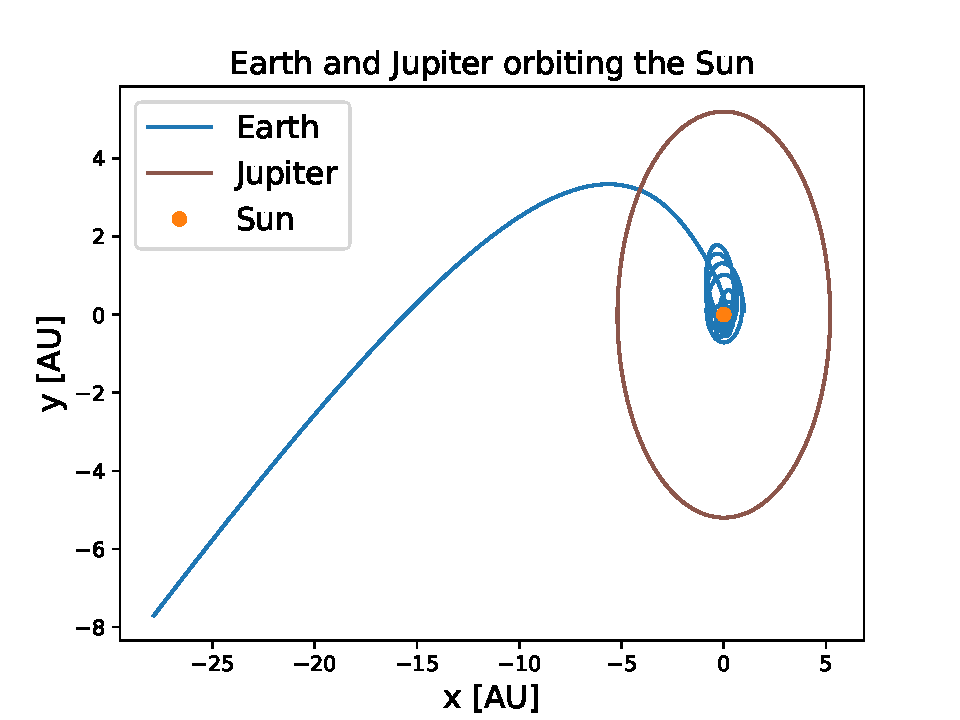
\includegraphics[scale=0.53]{3e-1000m-n1e3-t14.pdf}}
\subfloat{(a) This plot is for for $n = 1000$ points, the stability of Verlet is very low and it is apparent that interaction between any of the bodies result in large numerical errors.}
}\qquad
{{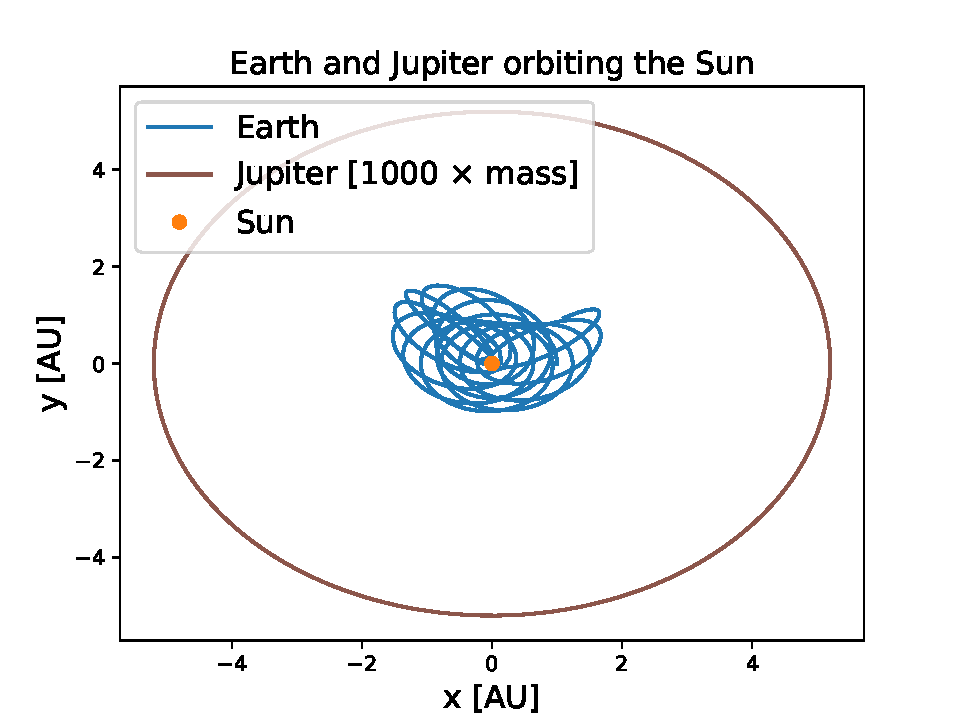
\includegraphics[scale=0.53]{3e-1000m-n1e6-t13.pdf}}
\subfloat{(b) This plot for $n = 10^{6}$ points, which is more stable.}
}\qquad
\caption{A plot of the three body problem solved for stationary Sun. The figure represents the Earth and Jupiter orbiting the sun for 13 Earth years, with Jupiter's mass being increased by a factor of 1000, we can see a drastic change in Earth's orbit.}
\label{fig:Jupiter1000}
\end{figure}

\subsection{Final model: Including all planets and Pluto}

\begin{figure}[t]
\mbox{\epsfig{figure=3f-n1e6-t25_zoom.pdf,width=\linewidth,clip=}}
\caption{Drift of COM of the Solar System when letting gravity affect the Sun. Avoiding a drift in the COM proved difficult, however the one shown in the figure was of order of magnitude $10^{-4}AU$.}
\label{fig:3f_zoom}
\end{figure}


\begin{figure}[H]
{{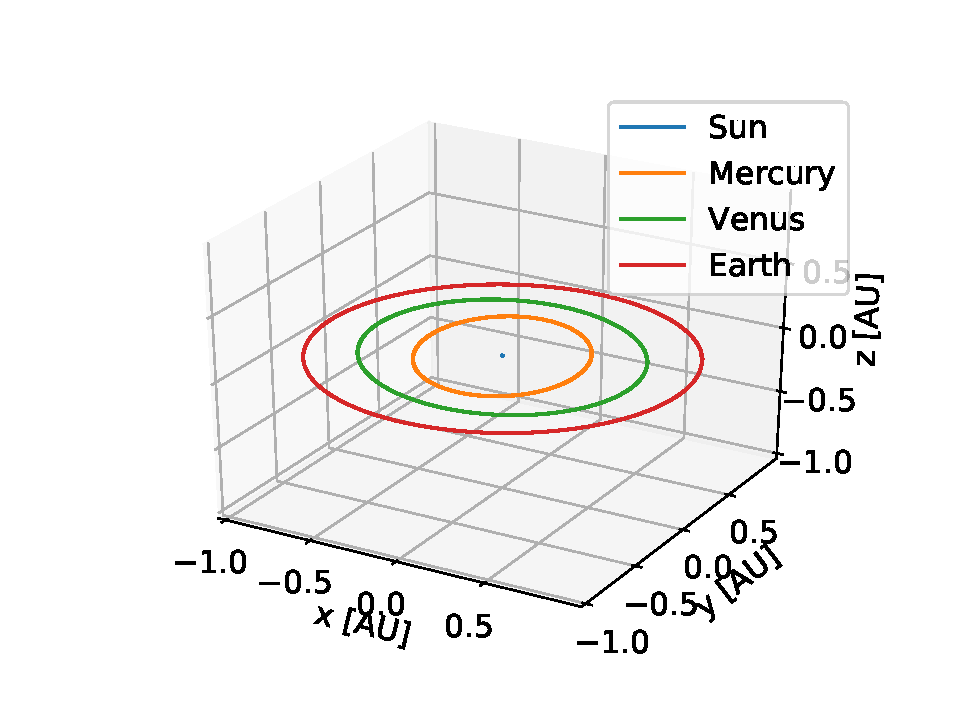
\includegraphics[scale=0.53]{inner3planets.pdf}}
\subfloat{(a) A 3d plot depicting the Sun and its three innermost planets in orbit for 1 Earth year.}
}\qquad
{{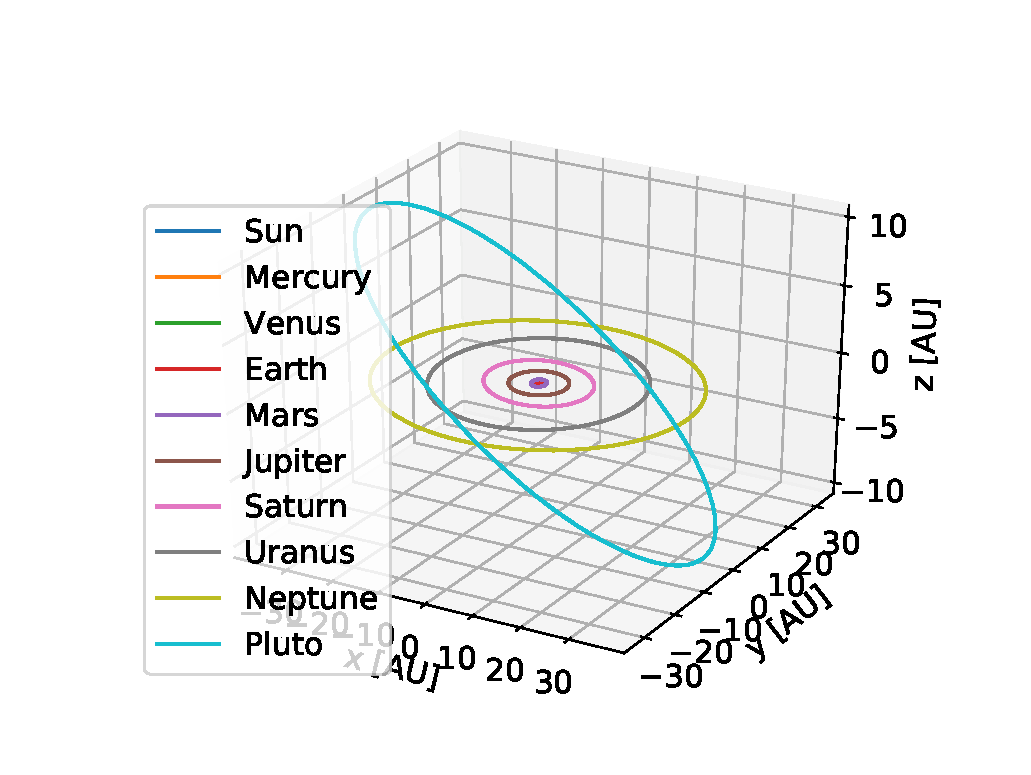
\includegraphics[scale=0.53]{solsys_full.pdf}}
\subfloat{(b) A 3d plot depicting all planets in the Solar System in orbit for 250 Earth years ensuring that Pluto completes its orbit.}
}\qquad
\caption{Plots of the Solar System in two different spatial and timescales, depiction includes all planets finishing at least one orbit.}
\label{fig:solsys}
\end{figure}

\begin{figure}[t]
\mbox{\epsfig{figure=3g-arcseconds.pdf,width=\linewidth,clip=}}
\caption{Perihelion precession of Murcery over 100 years.}
\label{fig:perihelion}
\end{figure}

\section{Discussion}
\label{sec:discussion}
\subsection{Stability and CPU-time of Euler compared to Verlet}
%
As seen in table \ref{tab:results1}, time complexity of Velocity Verlet is seemingly close to double compared to time complexity of Euler. This however is consistent with the number of FLOPS used for each of the methods as our Verlet algorithm seemingly runs at close to double the amount of FLOPS compared to Euler.
%
The Forward Euler method is clearly spiraling outwards as seen in figure \ref{fig:3c_euler}. This is a consequence of poor energy conservation shown in figure \ref{fig:energy_euler}. Using Euler-Cromer the energy conservation is much better as seen in figure \ref{fig:3c_eulercromer}. With the same time step and and simulation time the orbit remains seemingly constant. The same conservation of energy is also apparent when using the Velocity Verlet method as seen in figure \ref{fig:energy_verlet} when computing for shorter periods of time. As seen in fig.\ref{fig:mom_euler} Verlet even conserves angular momentum for shorter time periods.
%
Closed elliptic orbits are special cases of centripetal forces proportional to $1/r^2$. In figure \ref{fig:beta2'5} there is a change from $F_G \propto 1/r^2$ to $F_G \propto 1/r^{5/2}$ giving unstable orbits. When the force is changed with a $1/r^3$ proportionality the planet spirals out. The planet is no longer in a bound state and will over a relatively short time escape the Sun in its entirety.  


\subsection{Stability of Verlet introducing multiple bodies}

Adding another planetary body to our problem does not cause any visible destabilization in our Verlet method. However as the mass of this body increases beyond what is found among the planets of our Solar System the method destabilizes.

Increasing the mass of Jupiter does not only destabilize the orbit of Earth, it also destabilizes our Verlet method as the probability of the Earth coming too close to the Sun increases. This leads to numerical artifacts as a result of our step size being too short to reasonably simulate the next step in the resulting interaction between the Sun and Earth.

Pushing the three body problem further by letting gravity affect the Sun requires balancing of the total momentum done by moving the COM (centre of mass) to the center and setting the initial velocity so as to stop the COM from drifting. As seen in fig.\ref{fig:3f_zoom} the COM barely drifts when the Sun was in the initial condition explained above. However while the rest of the Planets will experience a similar drift the tiny order of magnitude prevents seeing any notable shifts in their orbits.

Even with Velocity Verlet the energy is not conserved completely over long periods of time. In figure \ref{fig:solsys}(b) the full Solar System is simulated over a period of 250 years. In this time the orbits of the innermost planets in particular have an energy drift. To get near perfect orbits the time steps must be infinitesimally small.


\subsection{Perihelion precession of Mercury}
As a final test of the stability of our numerical method as well as a test of natural phenomena explained by general relativity, the sturdiness of our model is tested by simulating the orbit of Mercury. Newtons gravitational force ($F_G \propto \frac{1}{r^{2}}$) is unable to describe the perihelion precession of Mercury, so to expand the model the relativistic correction in to the gravitational force (Eq. \eqref{eq:precession}) is introduced. Analyzing our results for the precession of Mercury as seen in \ref{fig:perihelion} we get $26''$ as compared to the reference value of $43''$. This result is not impressive either when considering that the error can not be accounted for by numerical errors only.



\section{Conclusions}
\label{sec:conclusions}

As demonstrated by the tests of numerical stability, the Velocity Verlet solver is clearly superior to the Euler solver when it comes to precision. When the Euler solver is used to compute the movement of a planet, the orbit quickly spirals out of its original shape. This shows that the Euler solver poorly conserves physical quantities such as the mechanical energy of the system. The Velocity Verlet method on the other hand conserves energy and momentum well with a slight trade off in the amount of FLOPS needed to preform the calculation.

The Euler-Cromer method seemingly also conserves energy quite well, but becomes more unstable at fewer integration points.

Lastly, even though our Verlet method failed the perihelion test it performed with overall reasonable stability when simulating the Solar System.



%\begin{figure}[t]
%
%\mbox{\epsfig{figure=filename.eps,width=\linewidth,clip=}}
%
%\caption{Description of figure -- explain all elements, but do not
%draw conclusions here.}
%\label{fig:figure_label}
%\end{figure}

\begin{acknowledgements}
  
\end{acknowledgements}

\begin{thebibliography}{}
\bibitem{bib:project3} Hjorth-Jensen, Morten, 2018, \textit{Project 3} \url{http://compphysics.github.io/ComputationalPhysics/doc/
Projects/2018/Project3/pdf/Project3.pdf} (24.10.18)

\bibitem{bib:nasa} \textit{HORIZONS Web Interface} \url{https://ssd.jpl.nasa.gov/horizons.cgi} (22.10.18)

\bibitem{bib:verlet} \textit{Verlet integration} \url{https://www.saylor.org/site/wp-content/uploads/2011/06/MA221-6.1.pdf} (24.10.18)
\end{thebibliography}


\end{document}
